\newpage
\section{Auswertung}
\subsection{Untersuchung des Lock-In-Verstärkers}
In Abbildung (\ref{fig:1}) befinden sich die Screenshots des Oszilloskops zur Untersuchung des Lock-In-Verstärkers bei Phasenverschiebung ohne Rauschen. 

\begin{figure}
  \centering
  \begin{subfigure}{0.3\textwidth}
      \centering
      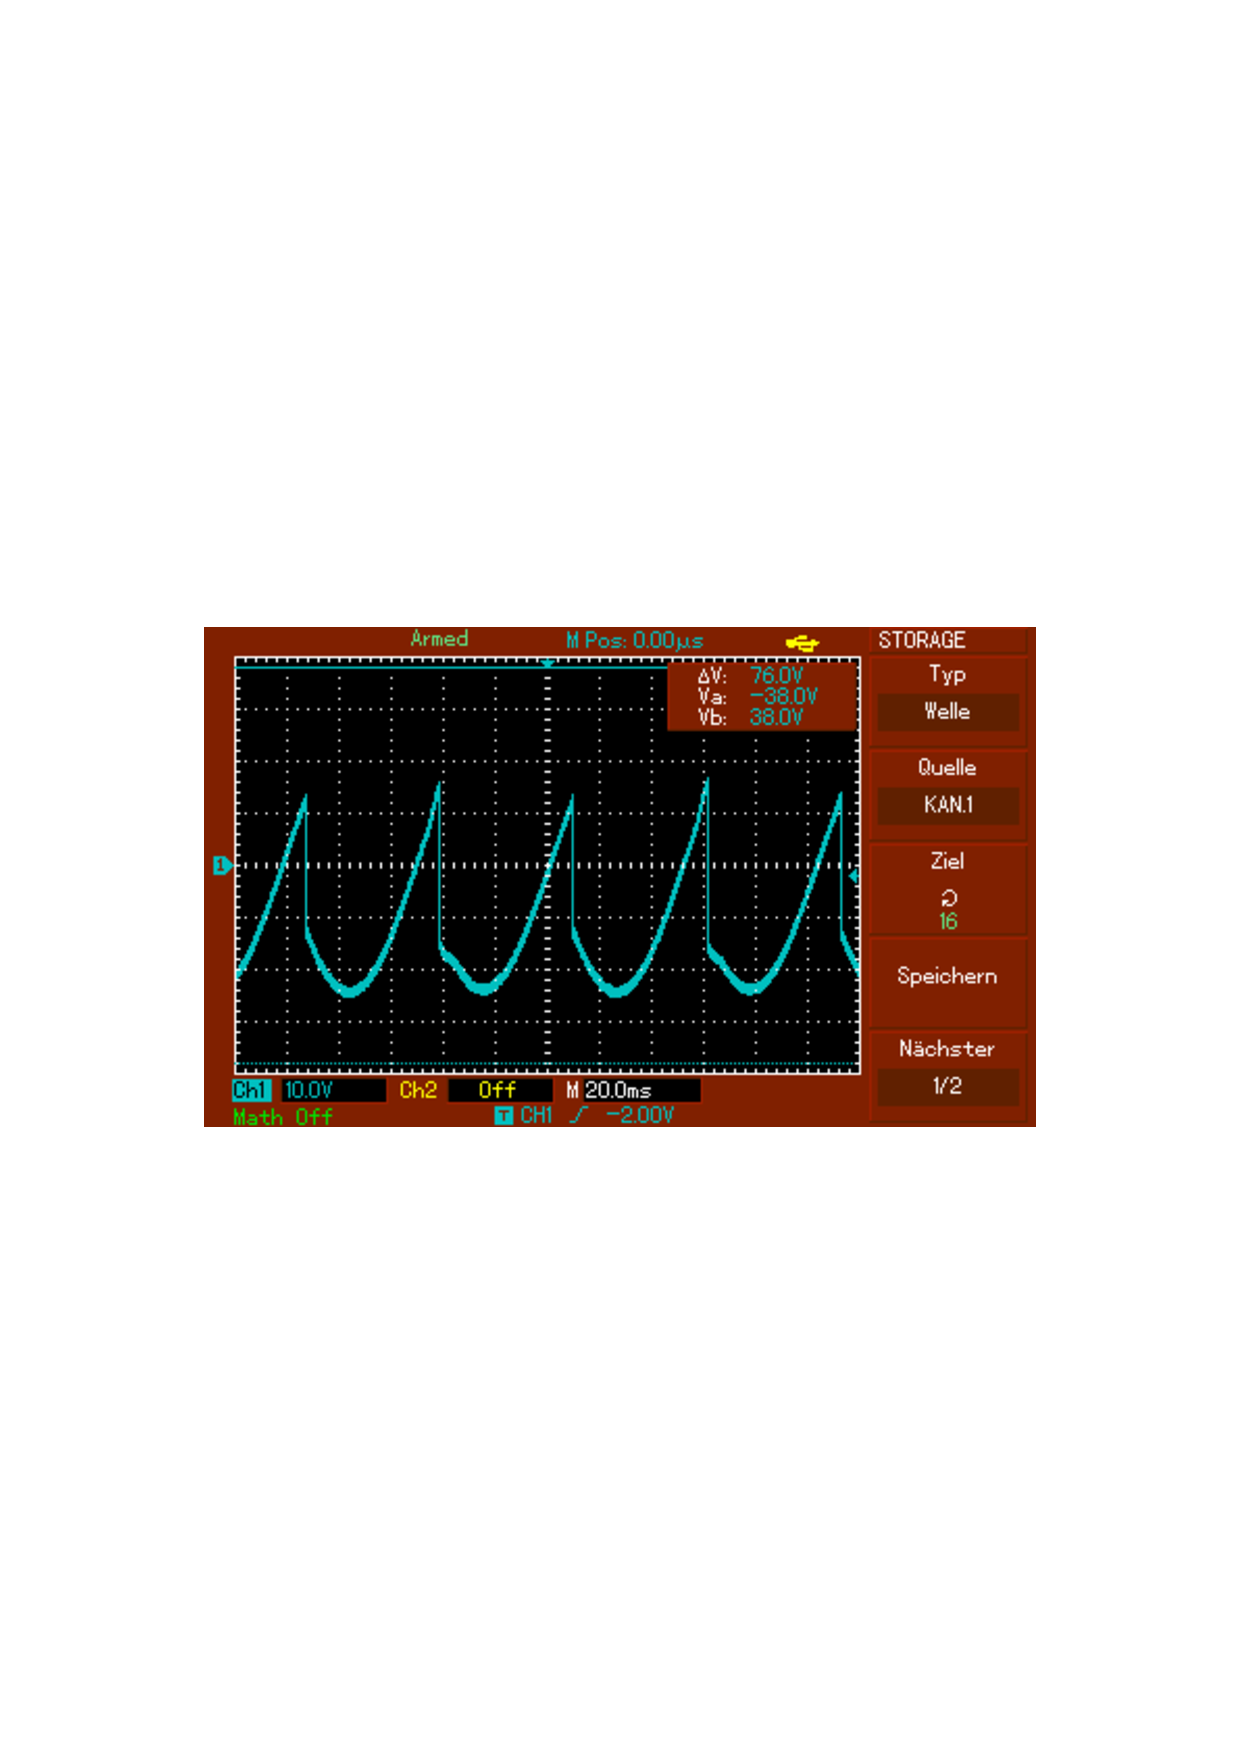
\includegraphics[width=\textwidth]{Daten/noNoise/0.pdf}
      \caption{$\phi = \SI{0}{\degree}$}
      \label{fig:0}
  \end{subfigure}
  \begin{subfigure}{0.3\textwidth}
      \centering
      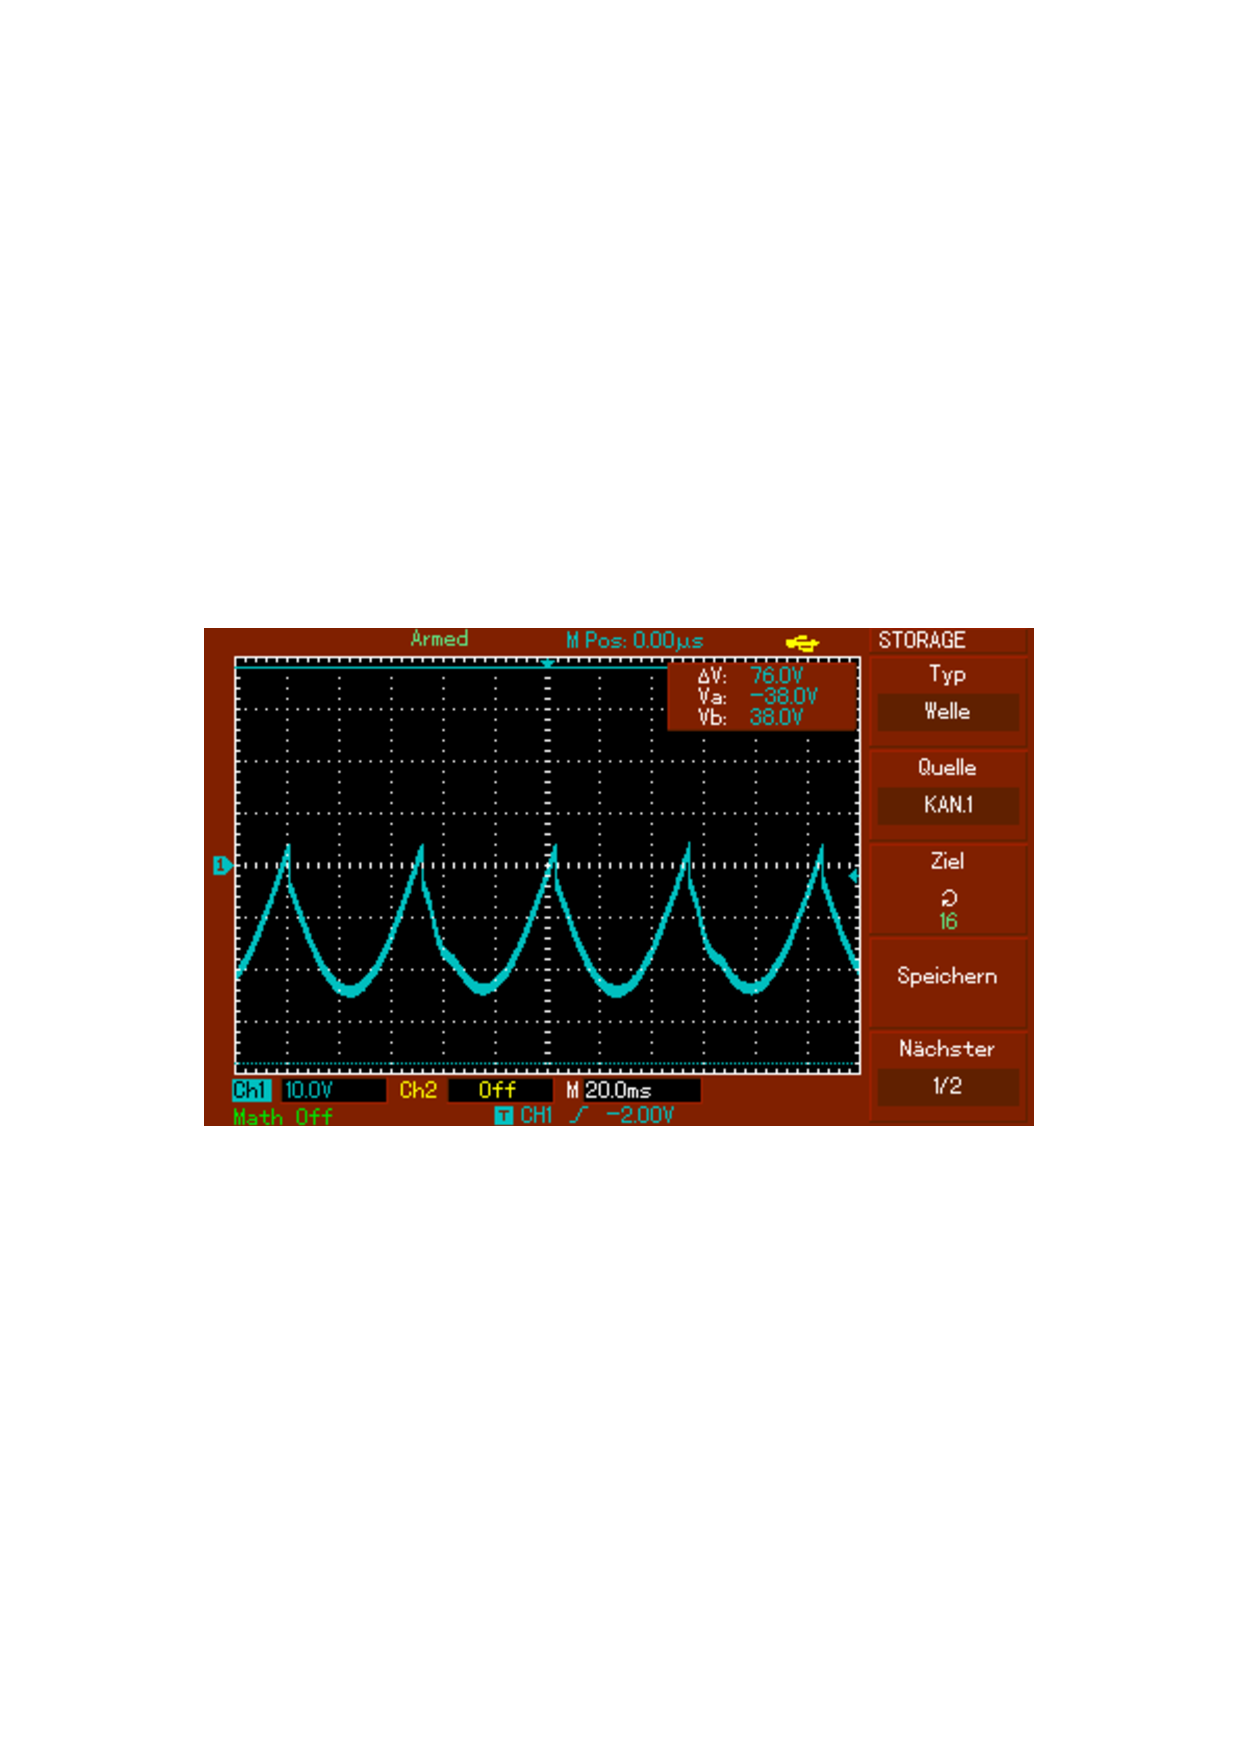
\includegraphics[width=\textwidth]{Daten/noNoise/30.pdf}
      \caption{$\phi = \SI{30}{\degree}$}
      \label{fig:1_45}
  \end{subfigure}
  \begin{subfigure}{0.3\textwidth}
      \centering
      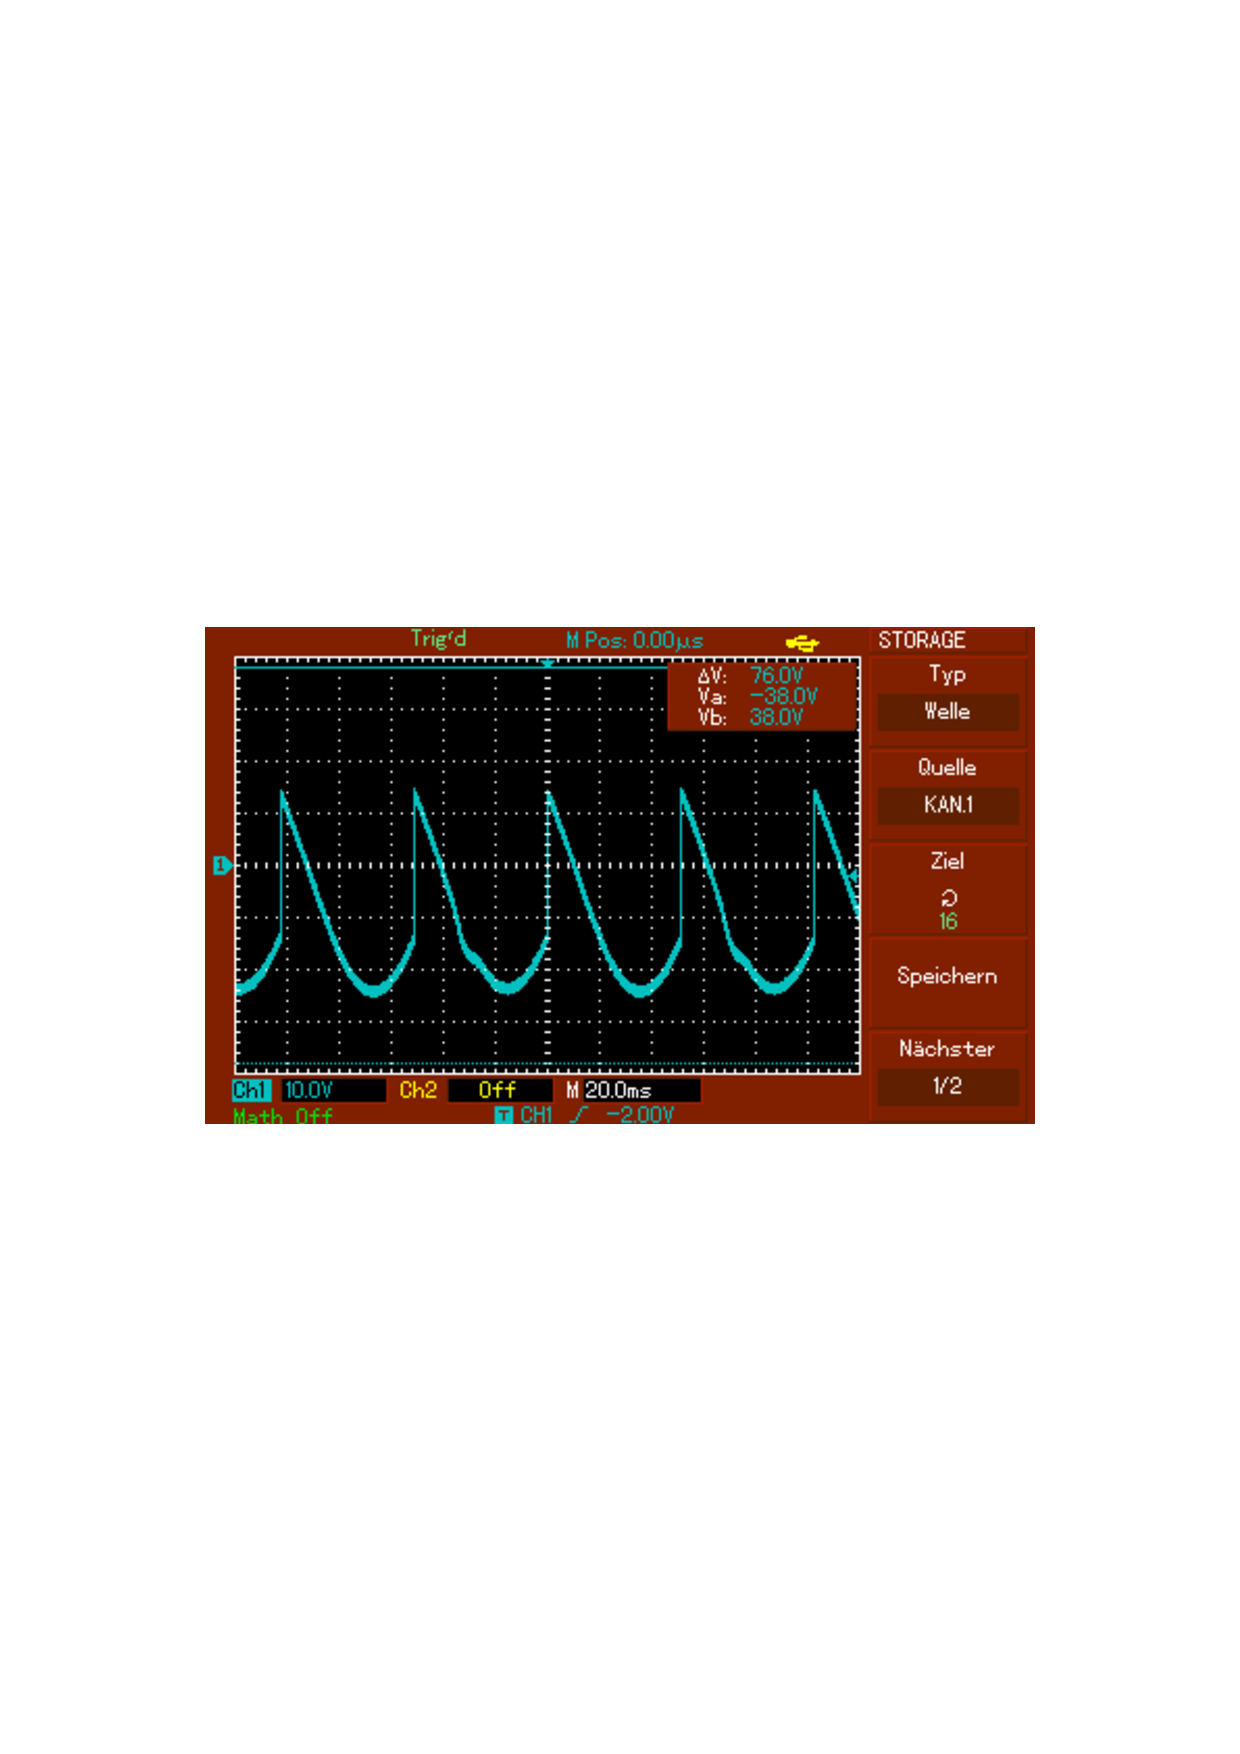
\includegraphics[width=\textwidth]{Daten/noNoise/60.pdf}
      \caption{$\varphi = \SI{60}{\degree}$}
      \label{fig:60}
  \end{subfigure}
  \par\medskip % Vertikaler Platz
  \begin{subfigure}{0.3\textwidth}
      \centering
      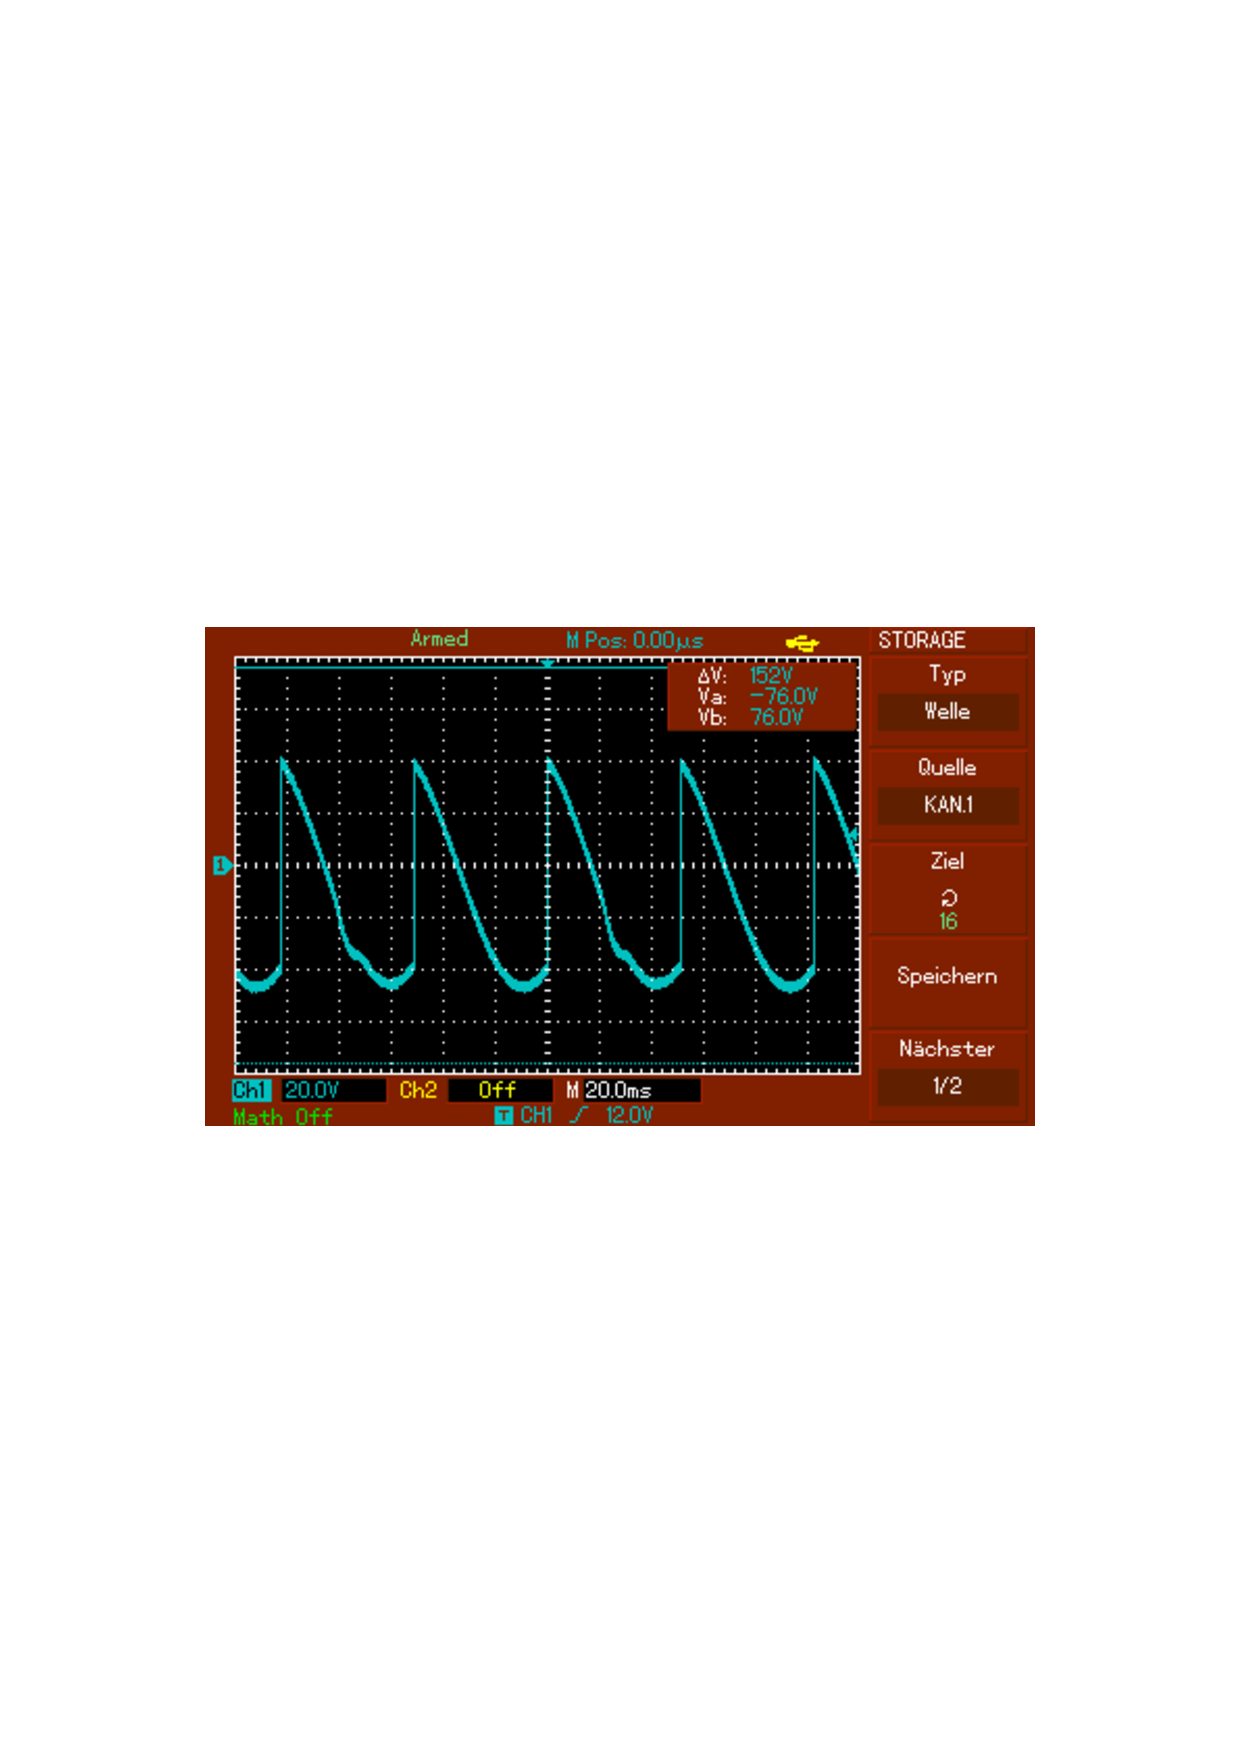
\includegraphics[width=\textwidth]{Daten/noNoise/90.pdf}
      \caption{$\phi = \SI{90}{\degree}$}
      \label{fig:90}
  \end{subfigure}
  \begin{subfigure}{0.3\textwidth}
      \centering
      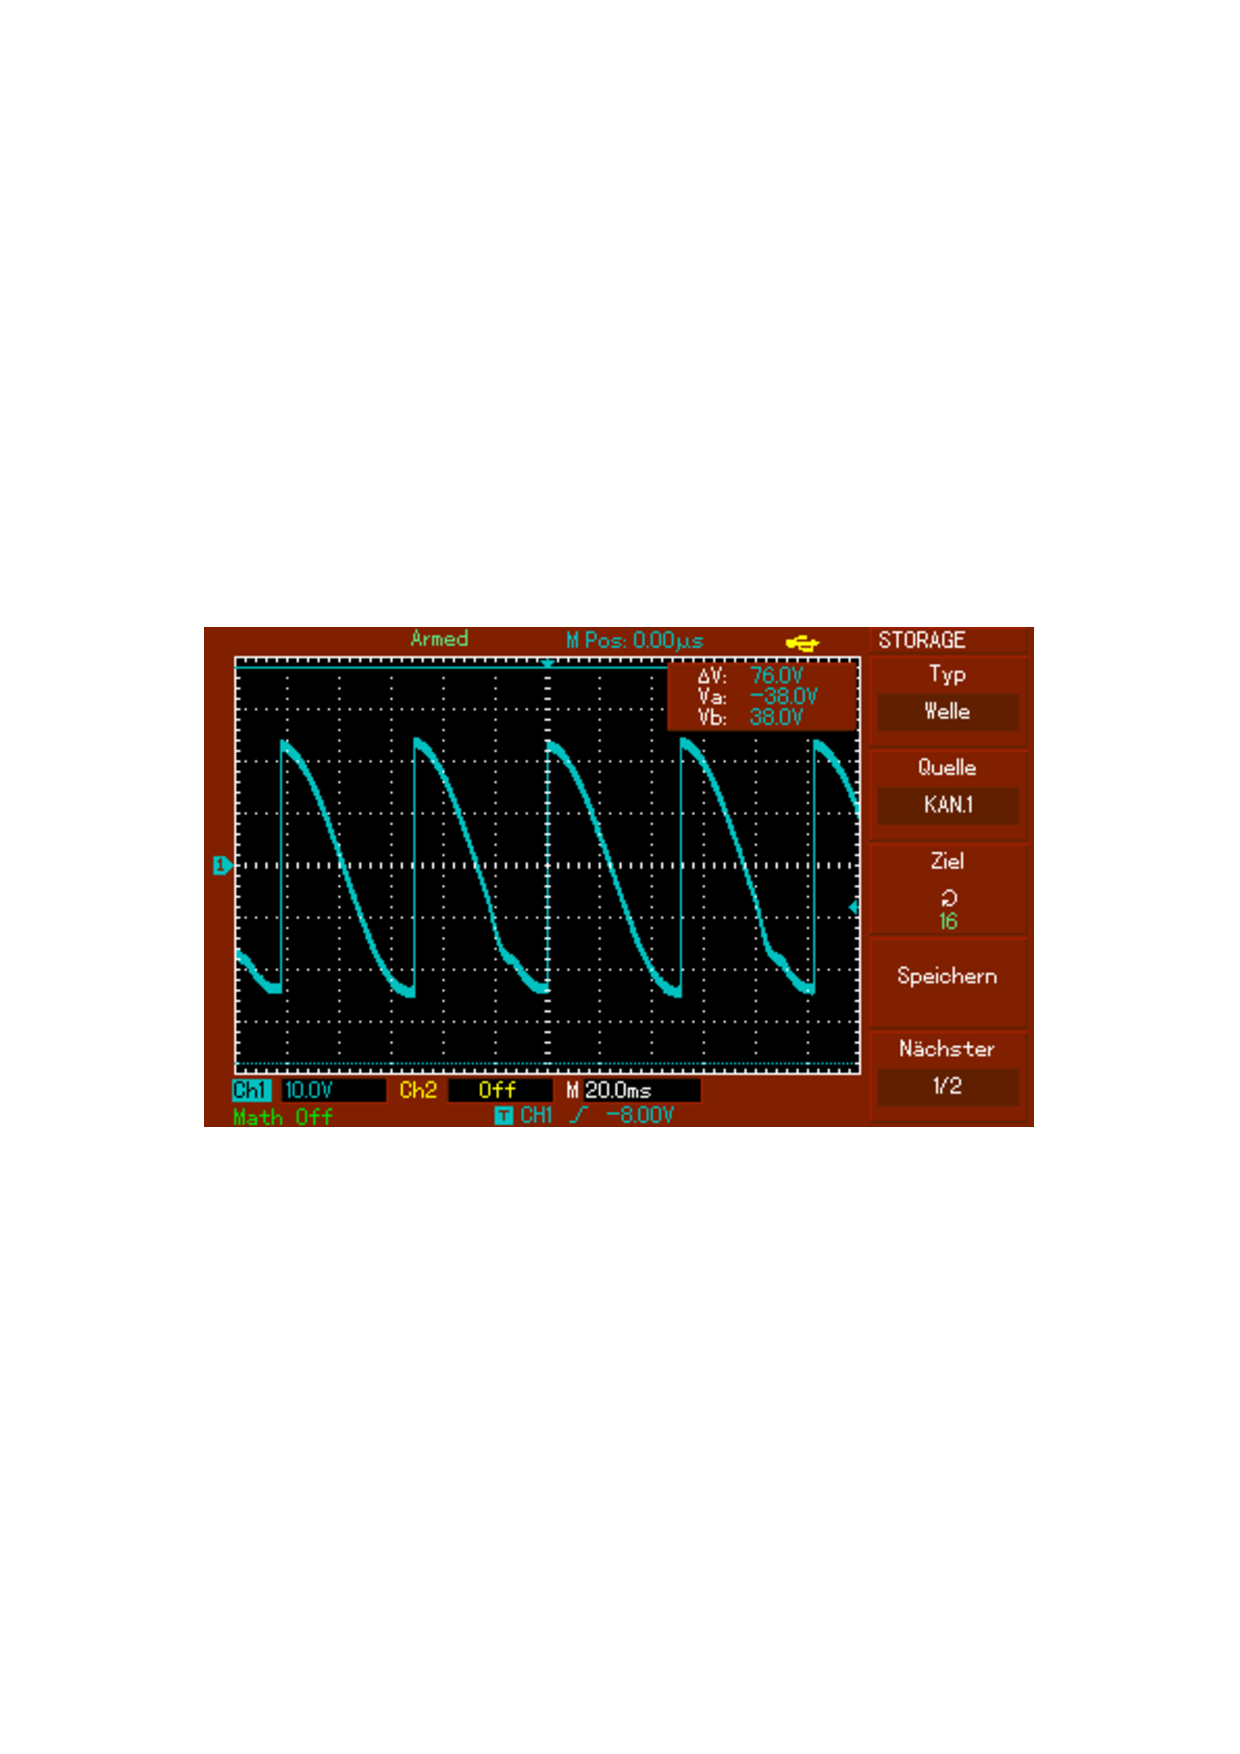
\includegraphics[width=\textwidth]{Daten/noNoise/120.pdf}
      \caption{$\phi = \SI{120}{\degree}$}
      \label{fig:120}
  \end{subfigure}
  \begin{subfigure}{0.3\textwidth}
      \centering
      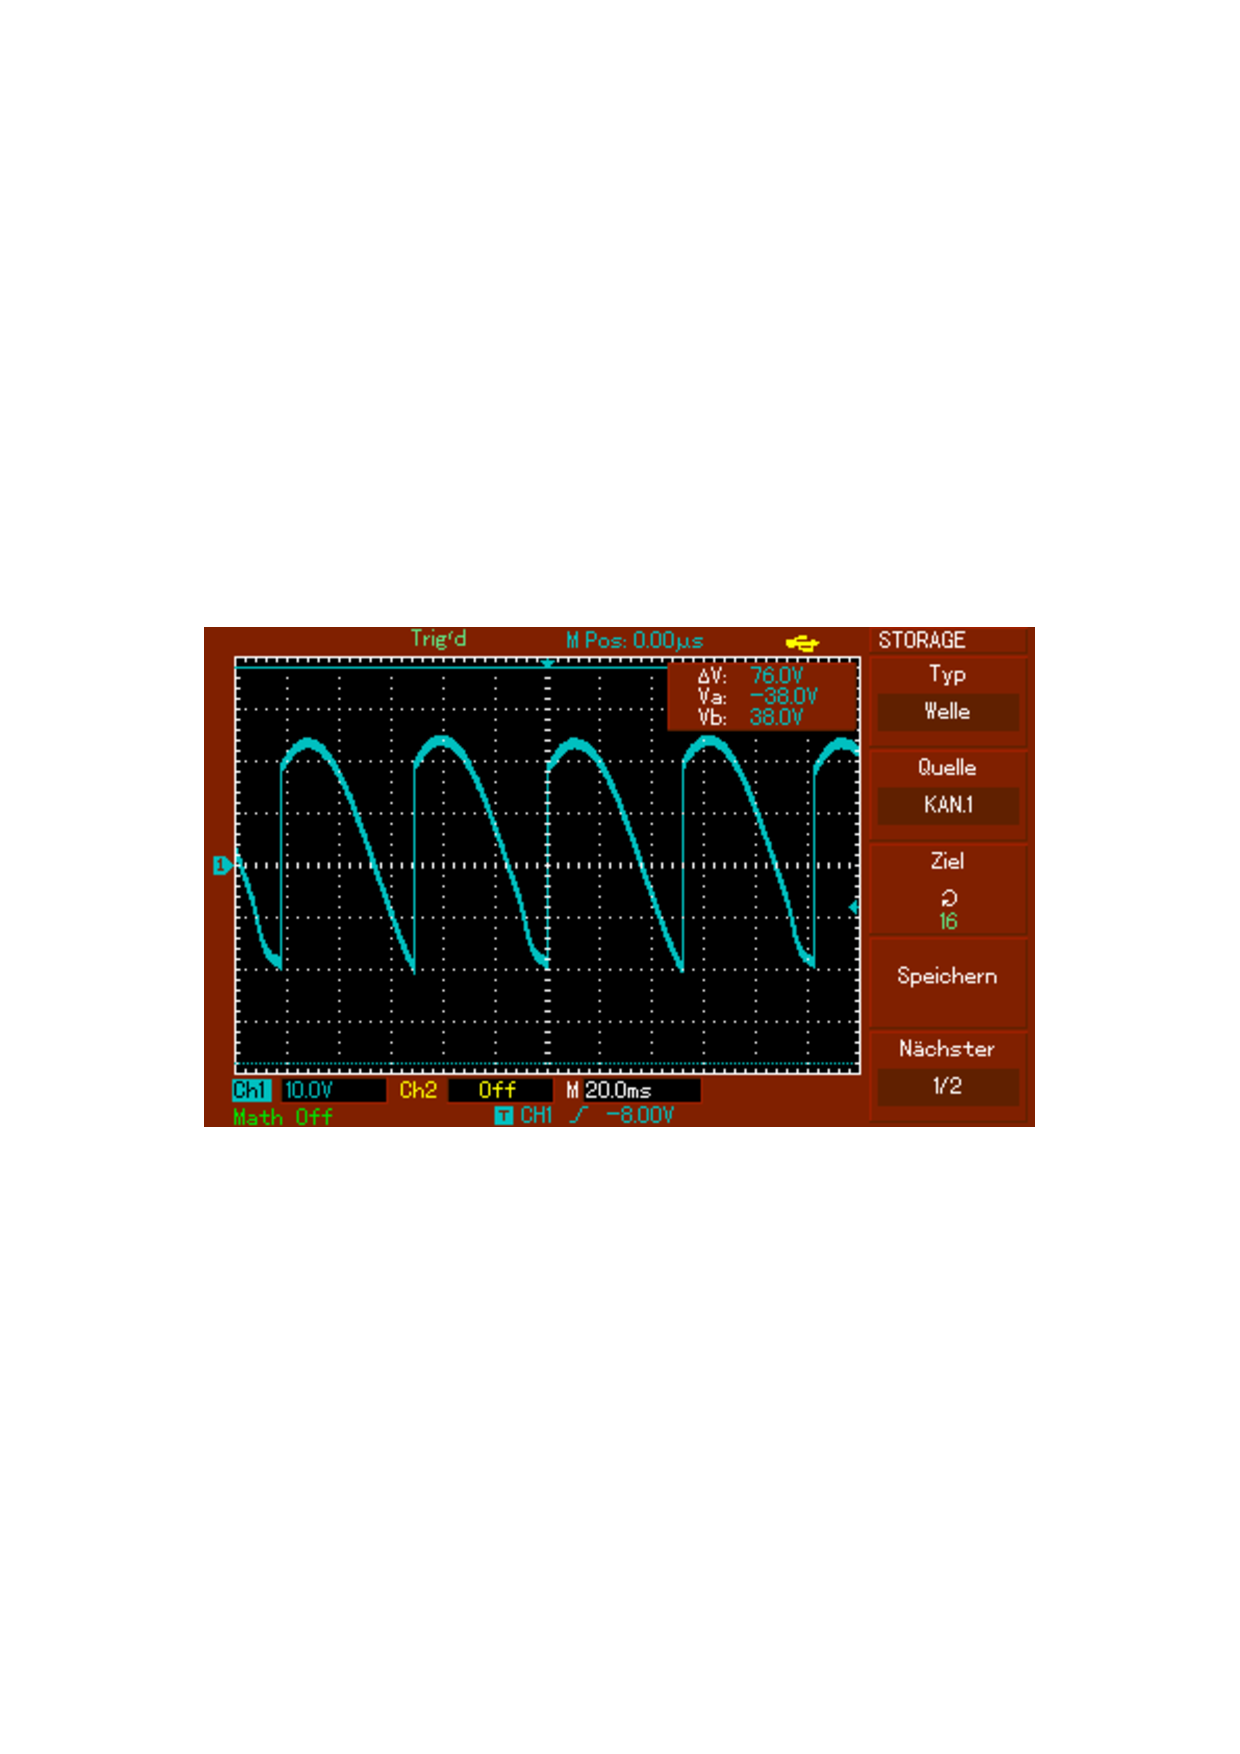
\includegraphics[width=\textwidth]{Daten/noNoise/150.pdf}
      \caption{$\phi = \SI{150}{\degree}$}
      \label{fig:150}
  \end{subfigure}
  \par\medskip % Vertikaler Platz
  \begin{subfigure}{0.3\textwidth}
      \centering
      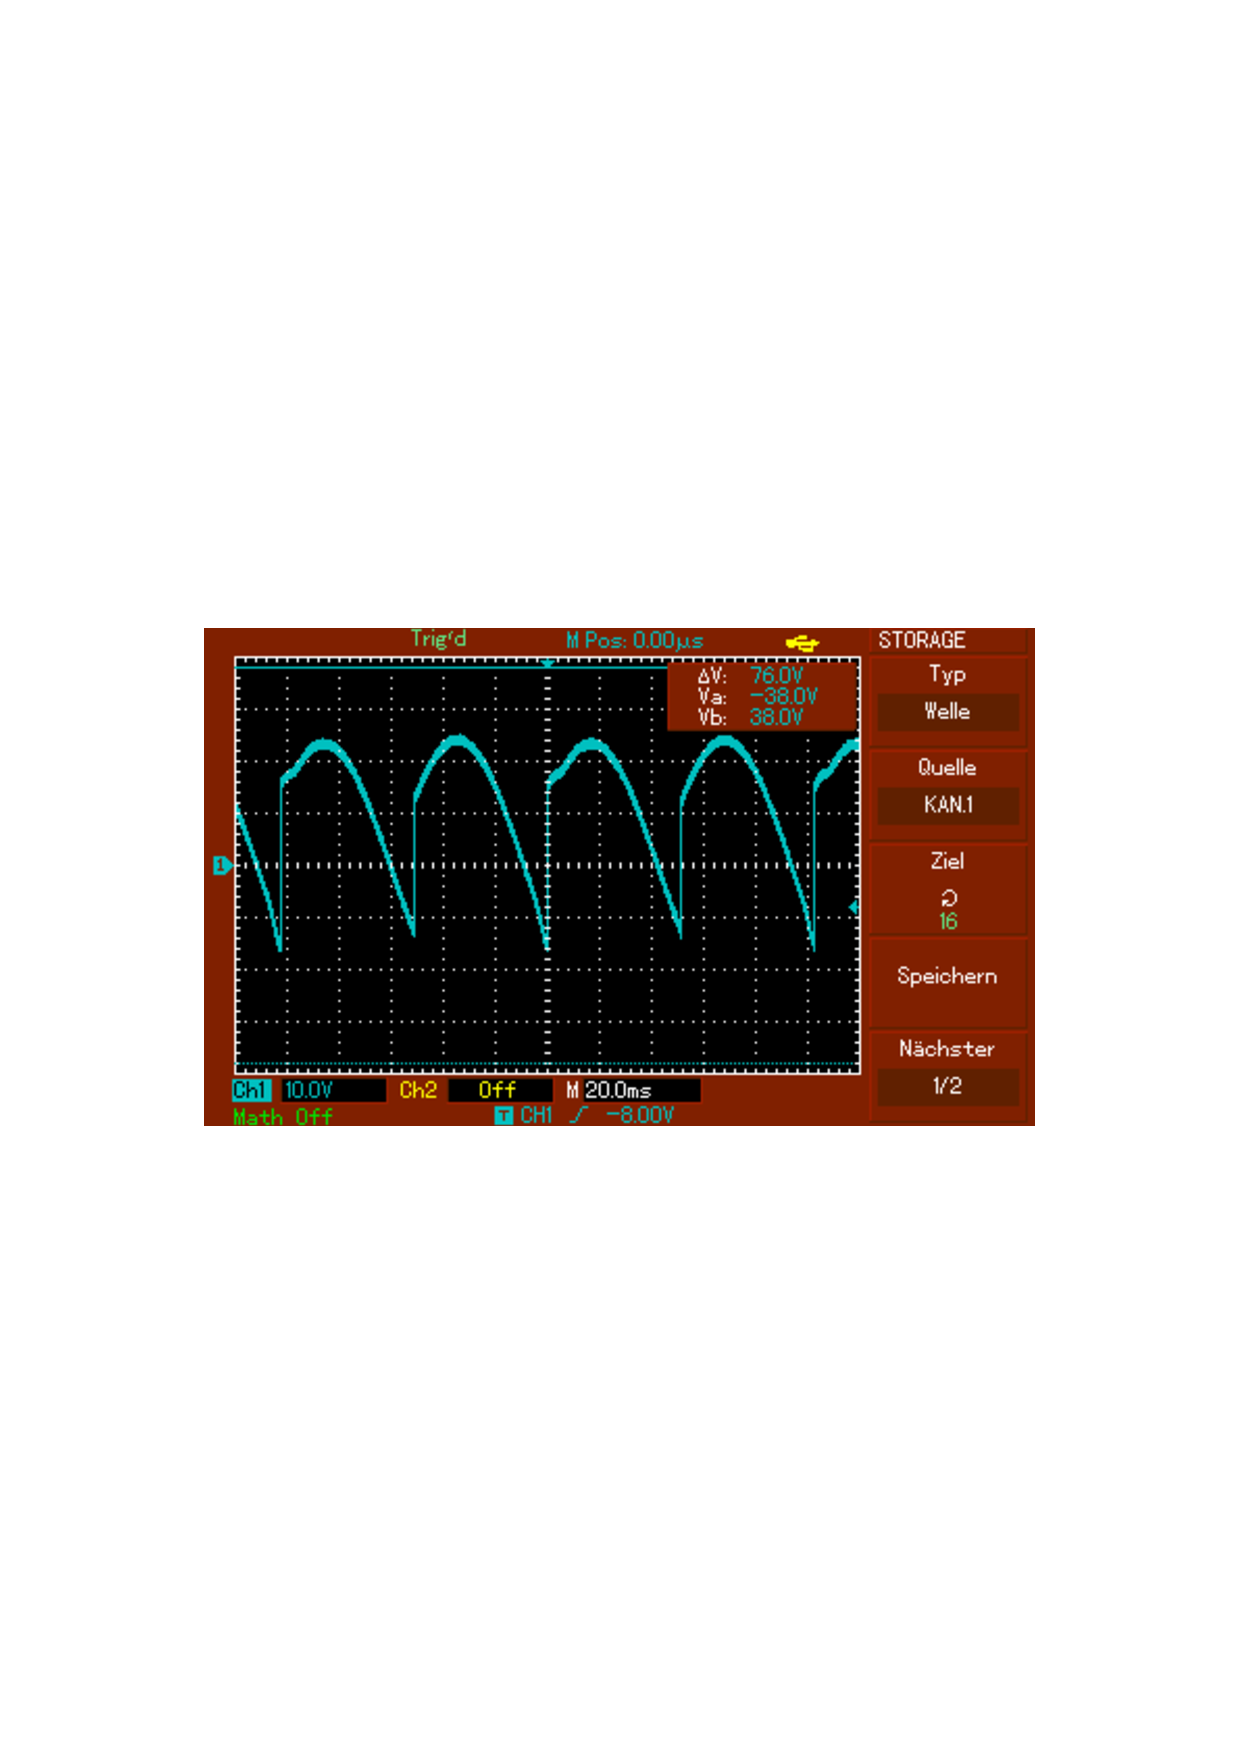
\includegraphics[width=\textwidth]{Daten/noNoise/180.pdf}
      \caption{$\phi = \SI{180}{\degree}$}
      \label{fig:180}
  \end{subfigure}
  \caption{Screenshots der Spannung ohne zwischengeschaltetem Noise-Generator bei verschiedenen Phasenverschiebungen $\phi$}
  \label{fig:1}
\end{figure}

\noindent
Analog befinden sich in Abbildung (\ref{fig:n}) die Bilder mit Rauschen.

\begin{figure}
  \centering
  \begin{subfigure}{0.3\textwidth}
      \centering
      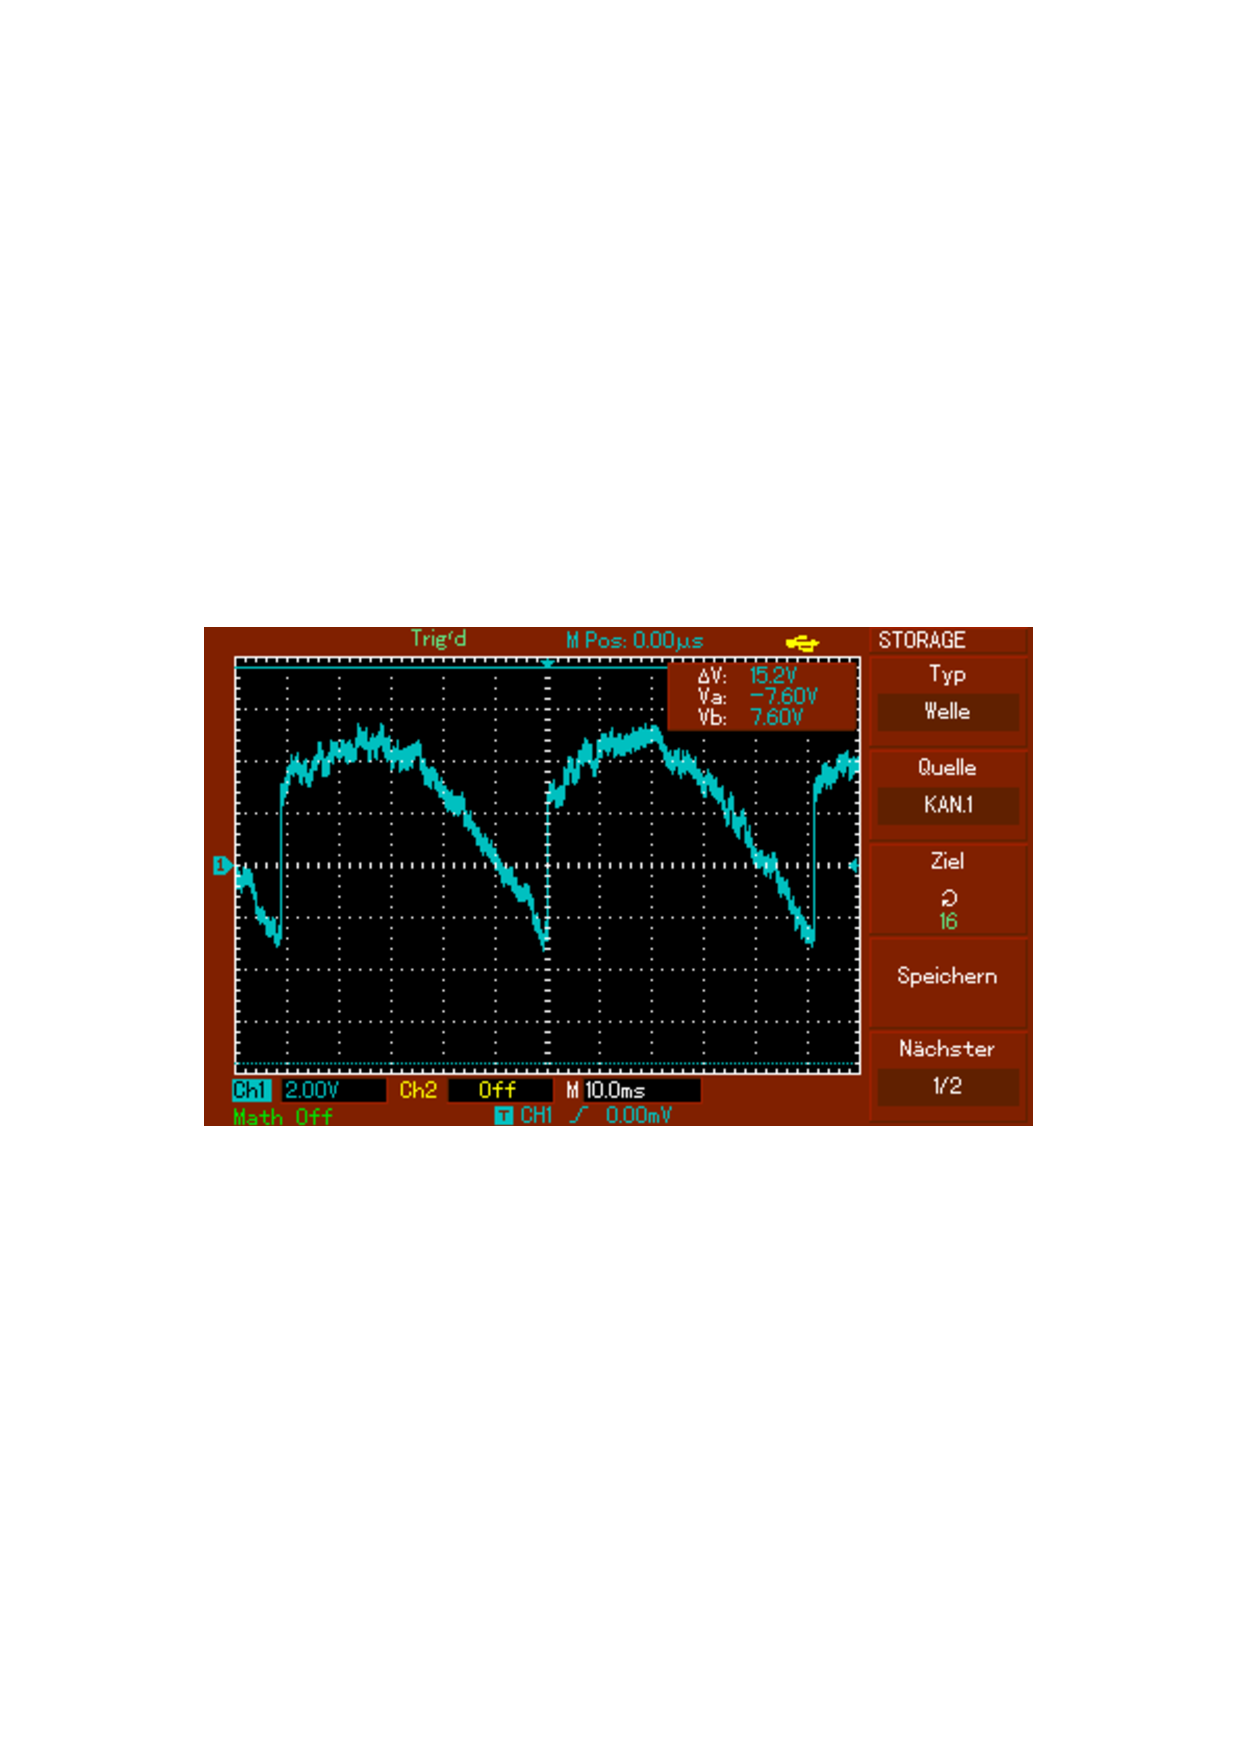
\includegraphics[width=\textwidth]{Daten/Noise/0.pdf}
      \caption{$\phi = \SI{0}{\degree}$}
      \label{fig:0n}
  \end{subfigure}
  \begin{subfigure}{0.3\textwidth}
      \centering
      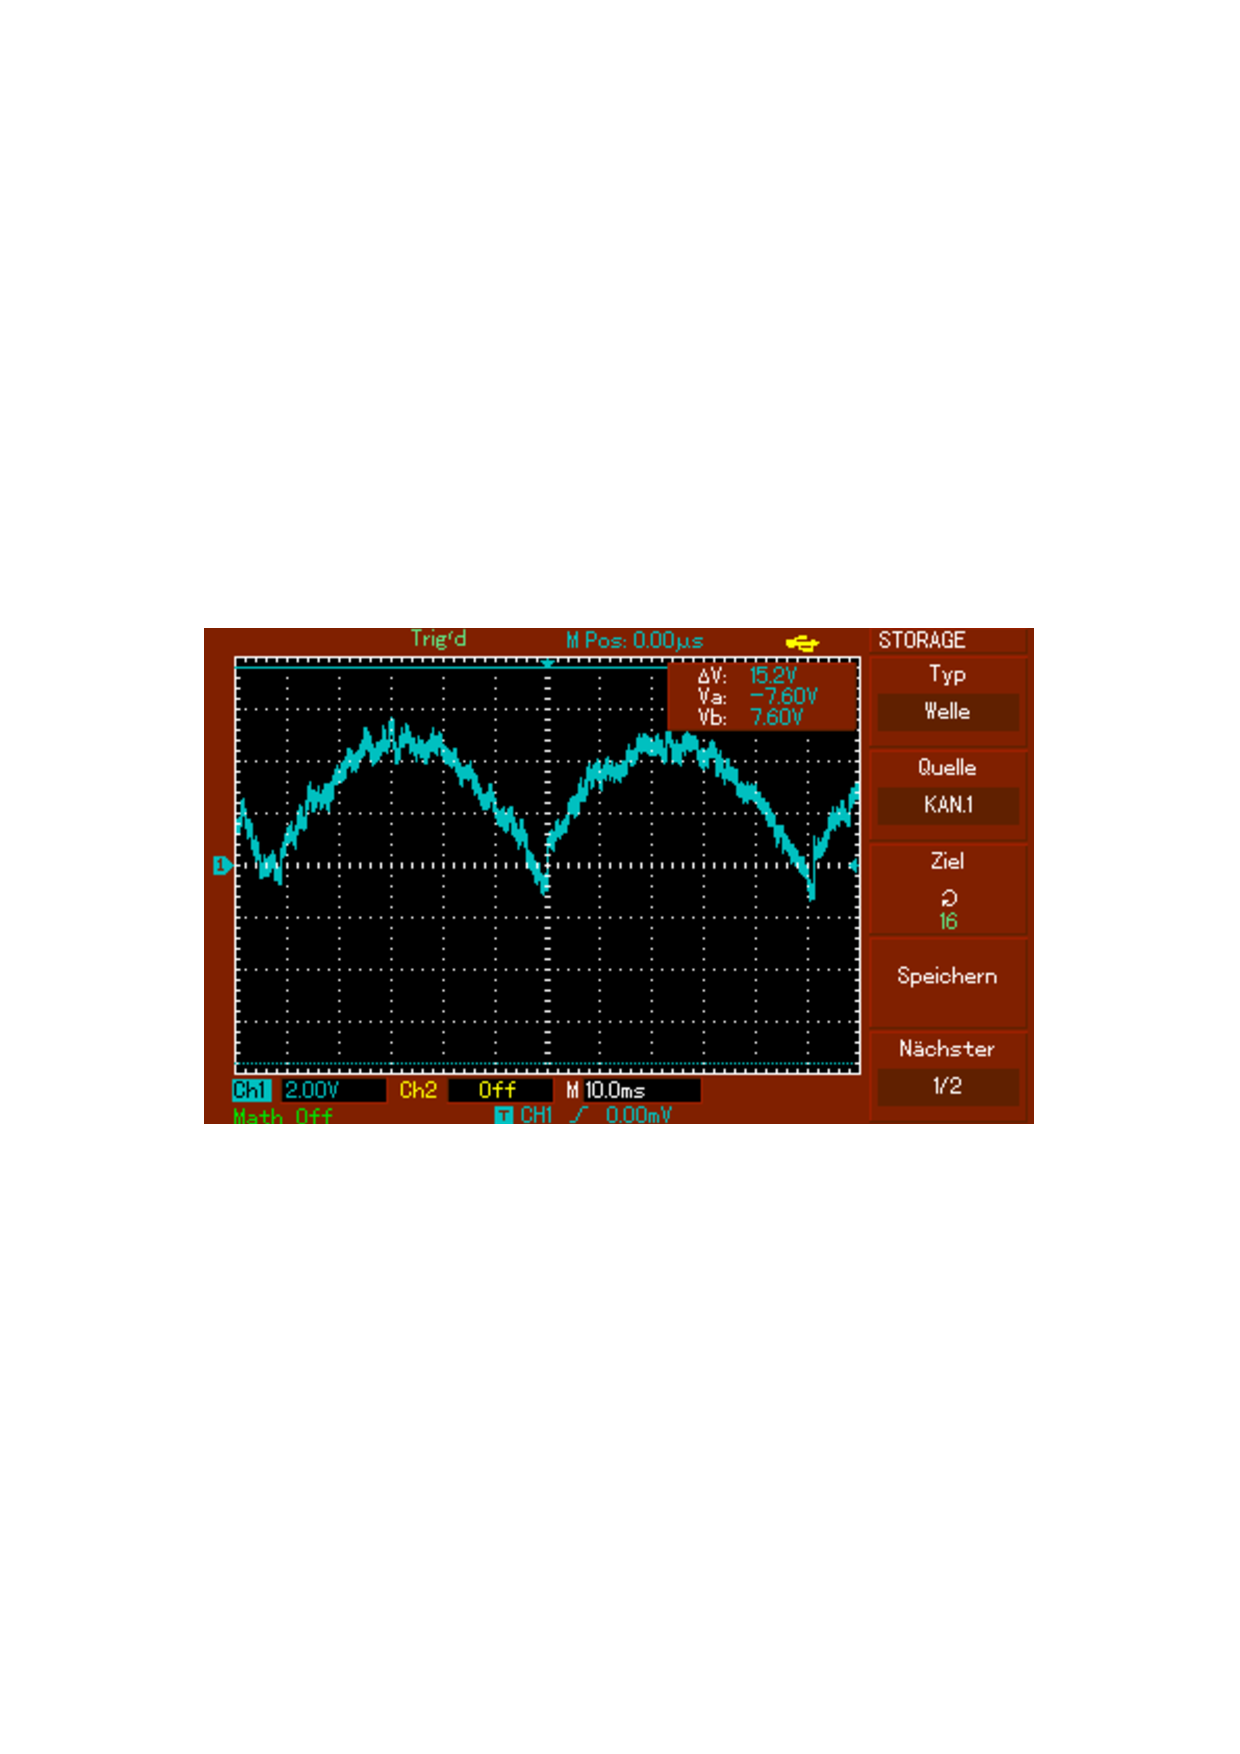
\includegraphics[width=\textwidth]{Daten/Noise/30.pdf}
      \caption{$\phi = \SI{30}{\degree}$}
      \label{fig:30n}
  \end{subfigure}
  \begin{subfigure}{0.3\textwidth}
      \centering
      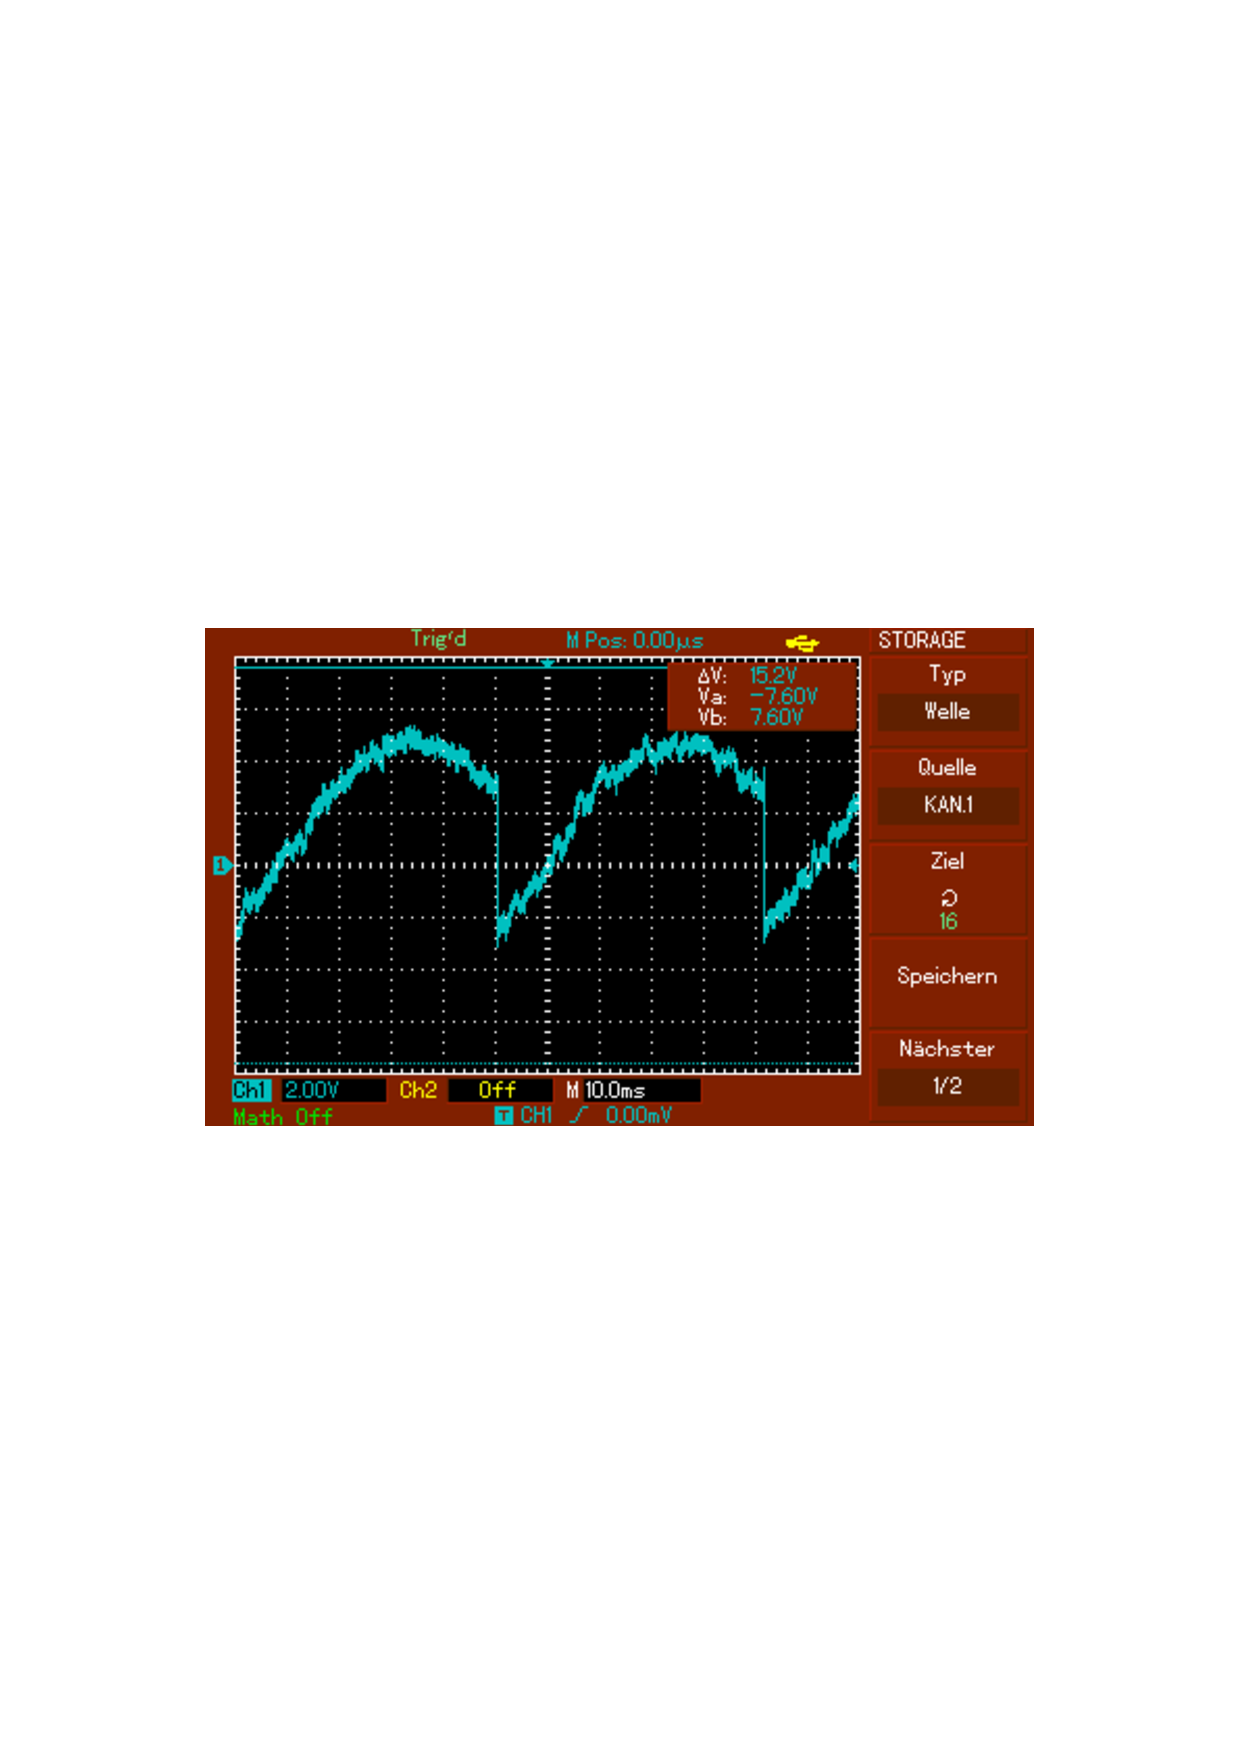
\includegraphics[width=\textwidth]{Daten/Noise/60.pdf}
      \caption{$\varphi = \SI{60}{\degree}$}
      \label{fig:60n}
  \end{subfigure}
  \par\medskip % Vertikaler Platz
  \begin{subfigure}{0.3\textwidth}
      \centering
      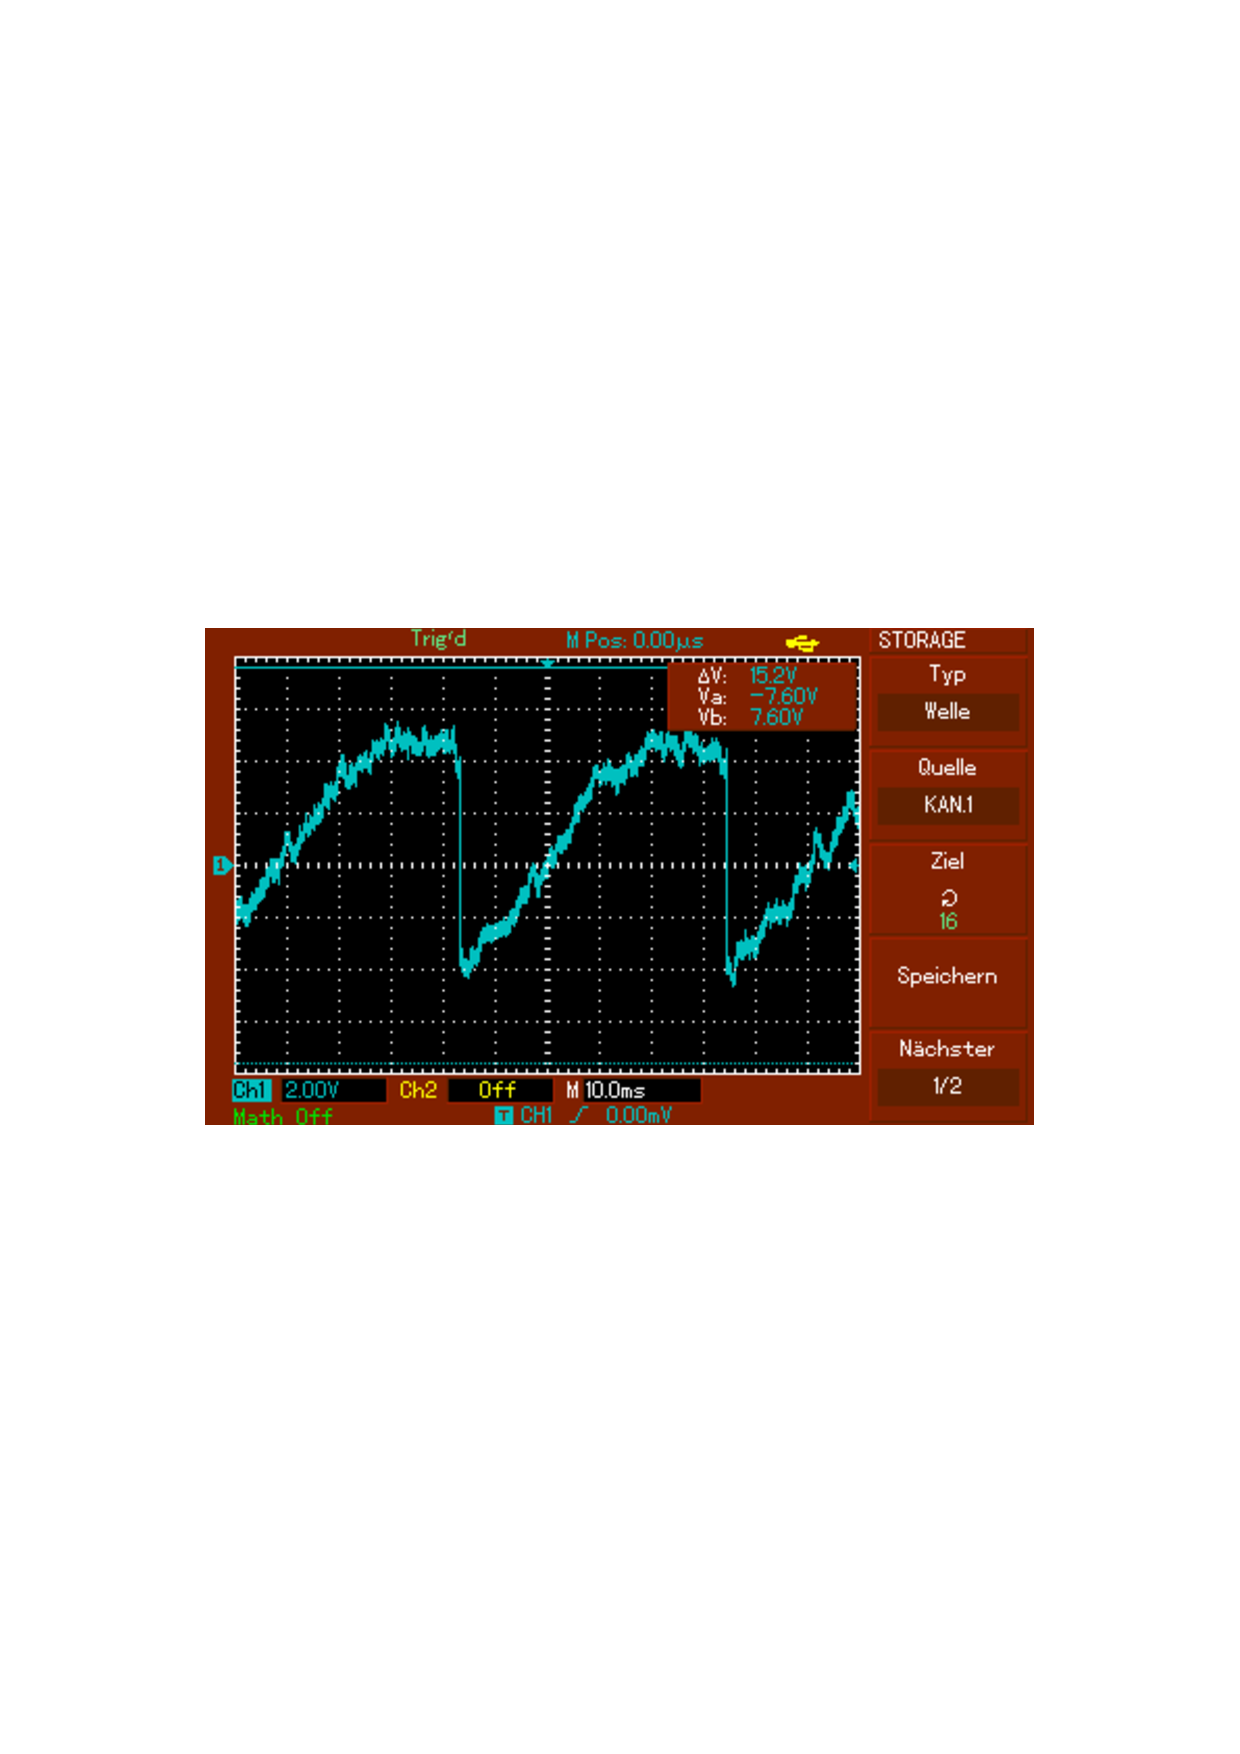
\includegraphics[width=\textwidth]{Daten/Noise/90.pdf}
      \caption{$\phi = \SI{90}{\degree}$}
      \label{fig:90n}
  \end{subfigure}
  \begin{subfigure}{0.3\textwidth}
      \centering
      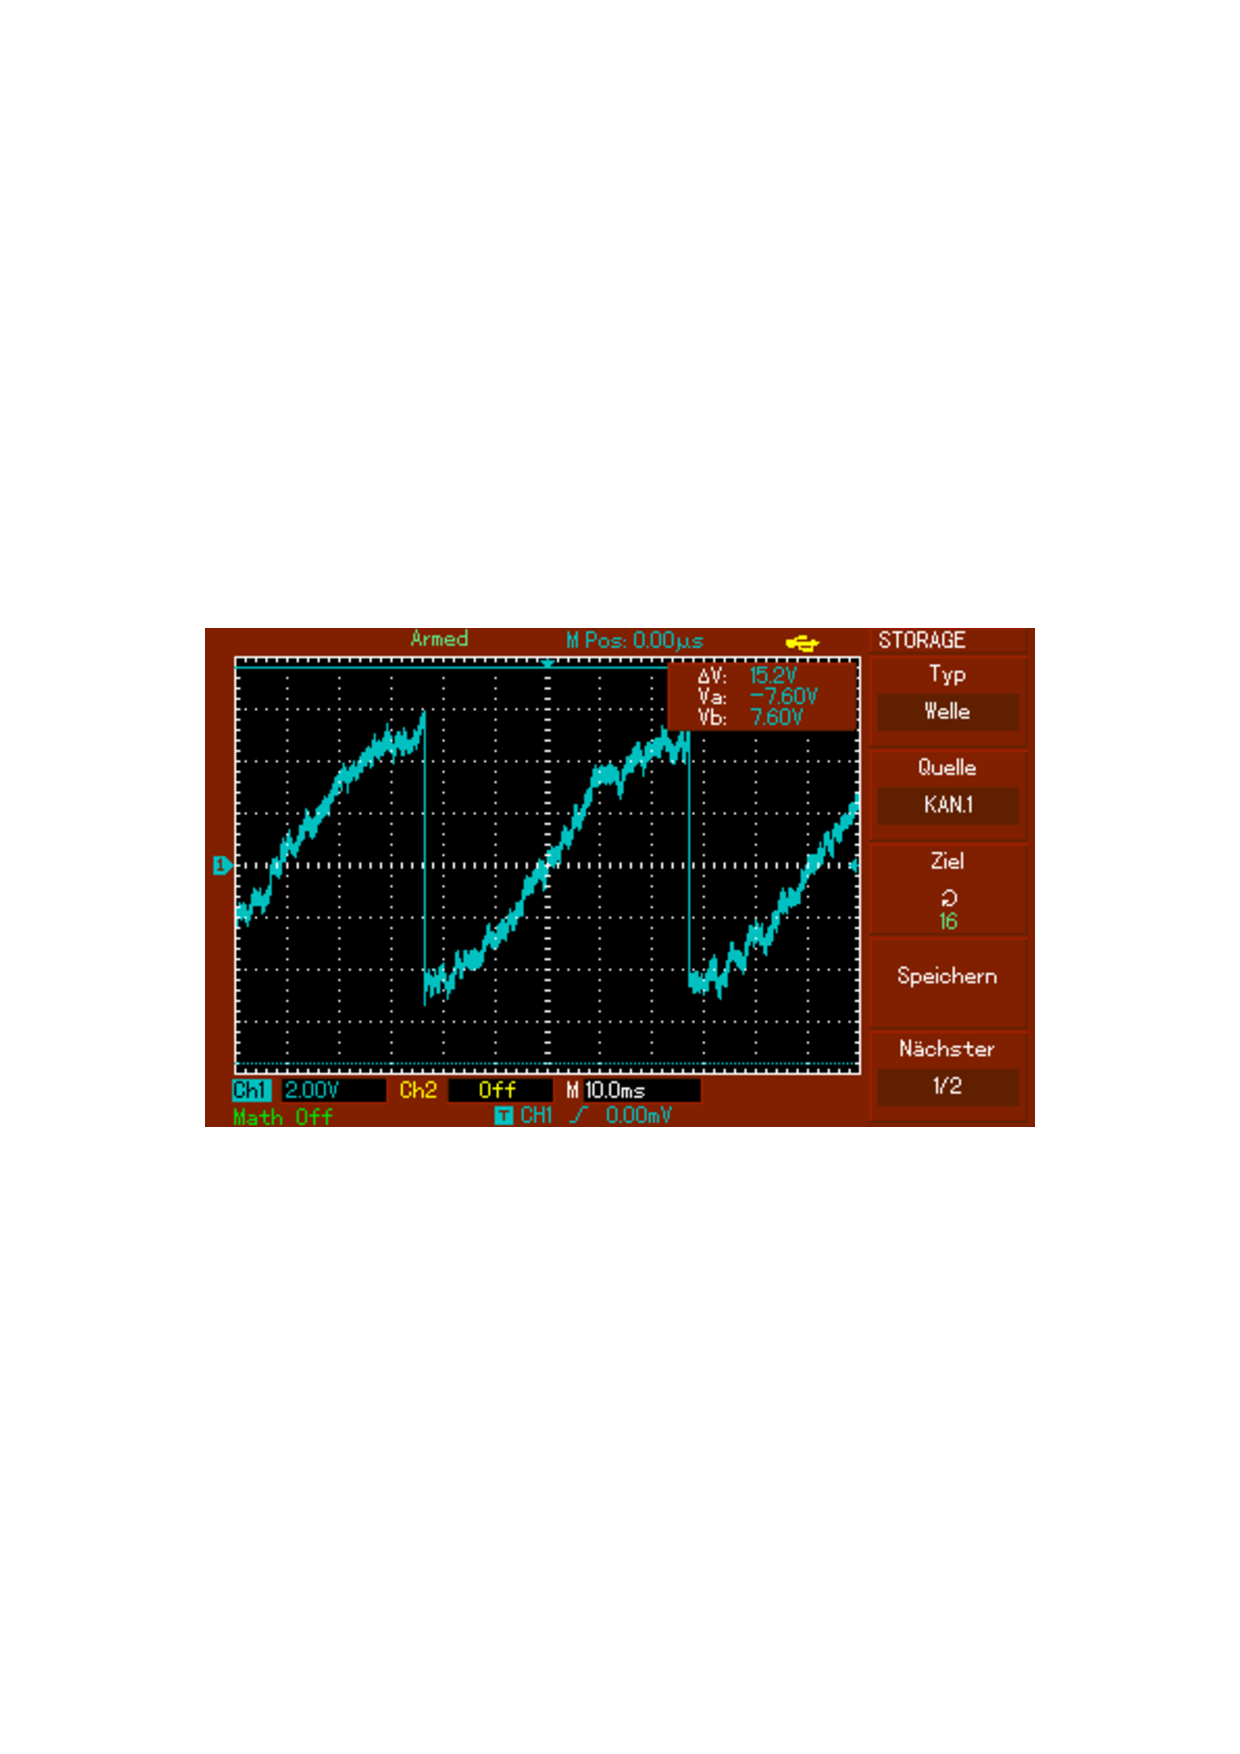
\includegraphics[width=\textwidth]{Daten/Noise/120.pdf}
      \caption{$\phi = \SI{120}{\degree}$}
      \label{fig:120n}
  \end{subfigure}
  \begin{subfigure}{0.3\textwidth}
      \centering
      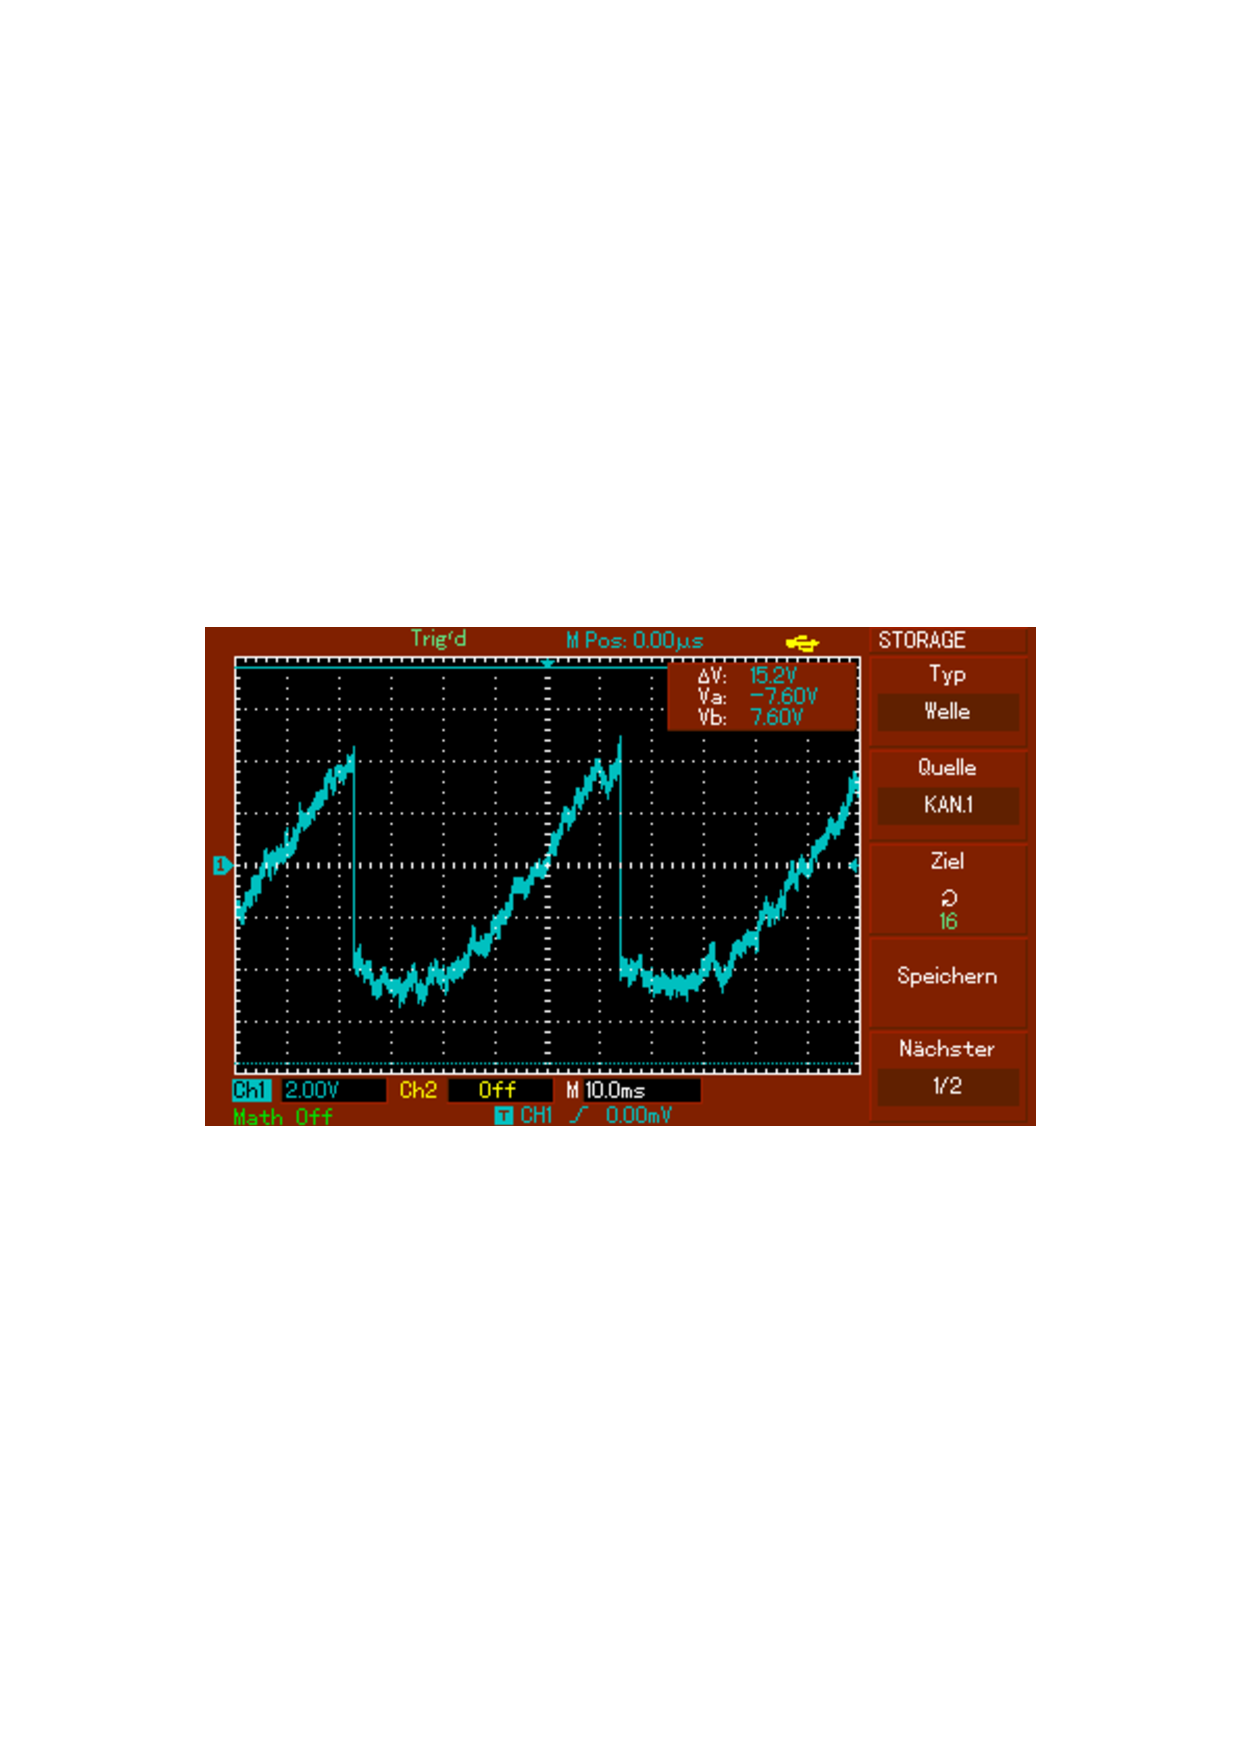
\includegraphics[width=\textwidth]{Daten/Noise/150.pdf}
      \caption{$\phi = \SI{150}{\degree}$}
      \label{fig:150n}
  \end{subfigure}
  \par\medskip % Vertikaler Platz
  \begin{subfigure}{0.3\textwidth}
      \centering
      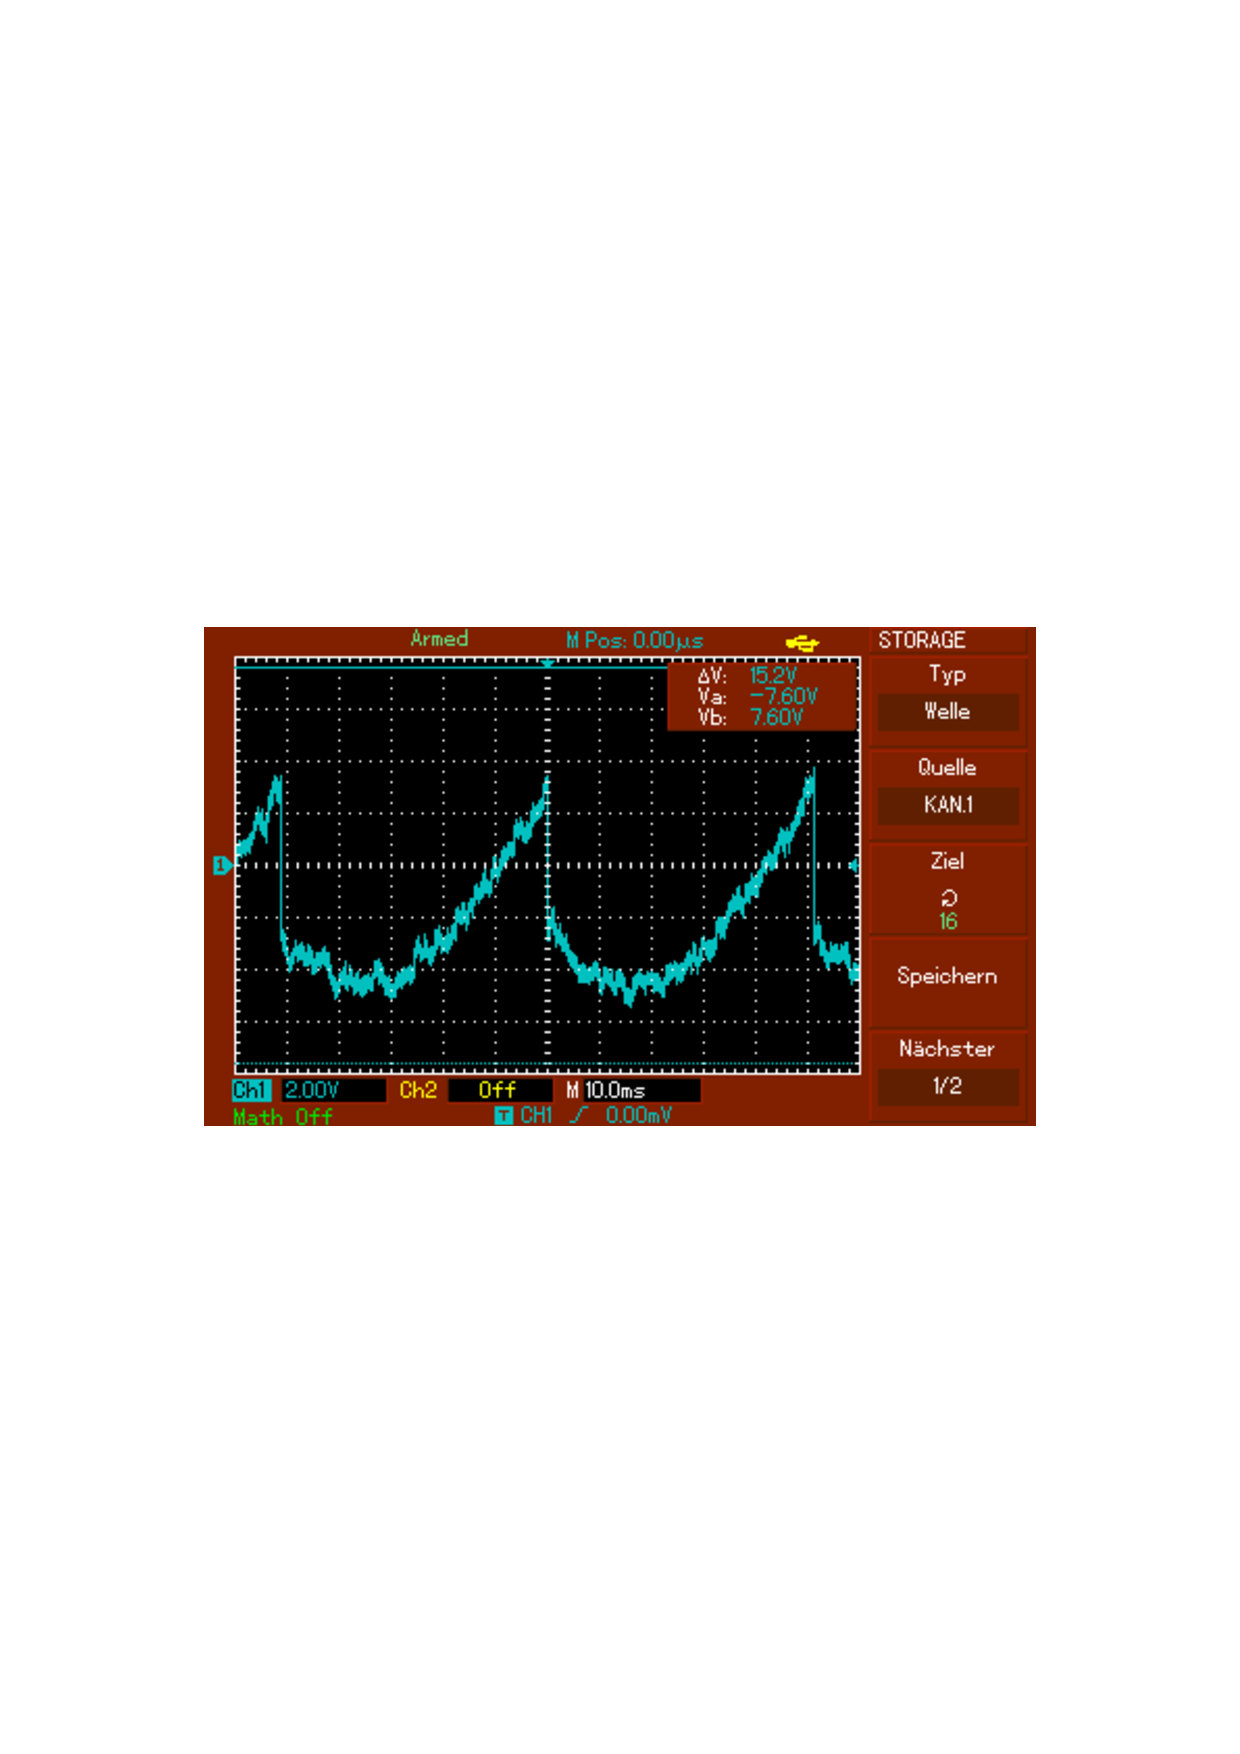
\includegraphics[width=\textwidth]{Daten/Noise/180.pdf}
      \caption{$\phi = \SI{180}{\degree}$}
      \label{fig:180n}
  \end{subfigure}
  \caption{Screenshots der Spannung mit zwischengeschaltetem Noise-Generator bei verschiedenen Phasenverschiebungen $\phi$}
  \label{fig:n}
\end{figure}

\noindent
Aus diesen Bildern ergeben sich die in Tabelle (\ref{tab:1}) aufgeführten Werte, wobei $U_o$ die Spannung ohne Rauschen
und $U_m$ die Spannung mit Rauschen darstellt.

\begin{table}
  \centering
  \begin{tabular}{c c c}
  \toprule
  {$\phi \mathbin{/} ° $} & {$U_o \mathbin{/} \si{\volt} $} &{$U_m \mathbin{/} \si{\volt} $}\\
  \midrule
  0   &    30  &     5  \\
  30  &    5   &     1.5\\
  60  &   -29  &     -6\\
  90  &   -80  &     -8\\
  120 &   -45  &     -11\\
  150 &   -40  &     -9\\
  180 &   -30  &     -6\\
  \bottomrule
  \end{tabular}
  \caption{Spannungsamplituden ohne und mit Rauschen in Abhängigkeit von $\phi$.}
  \label{tab:1}
  \end{table}

\newpage

\noindent
Werden die Spannungen in Abhängigkeit von der Phasenverschiebung aufgetragen, ergeben sich die Plots (\ref{fig:phase}) und (\ref{fig:phasenoise}).

\begin{figure}
  \centering
  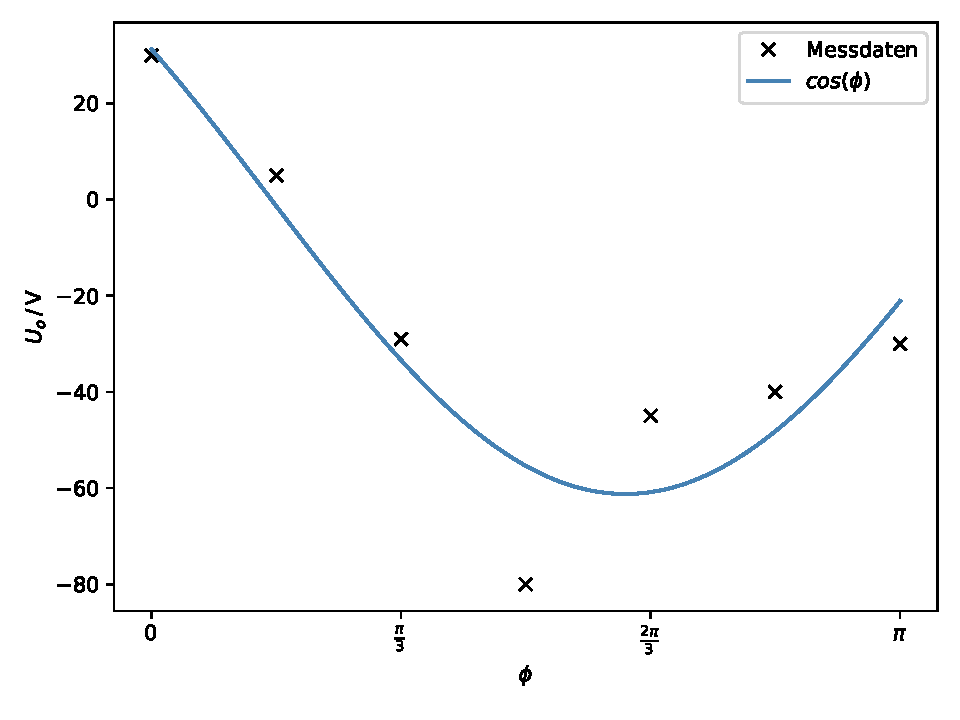
\includegraphics[height=6.9cm]{Daten/phase.pdf}
  \caption{Spannungsamplituden in Abhängigkeit von $\phi$ ohne Rauschen.}
  \label{fig:phase}
\end{figure}

\begin{figure}
  \centering
  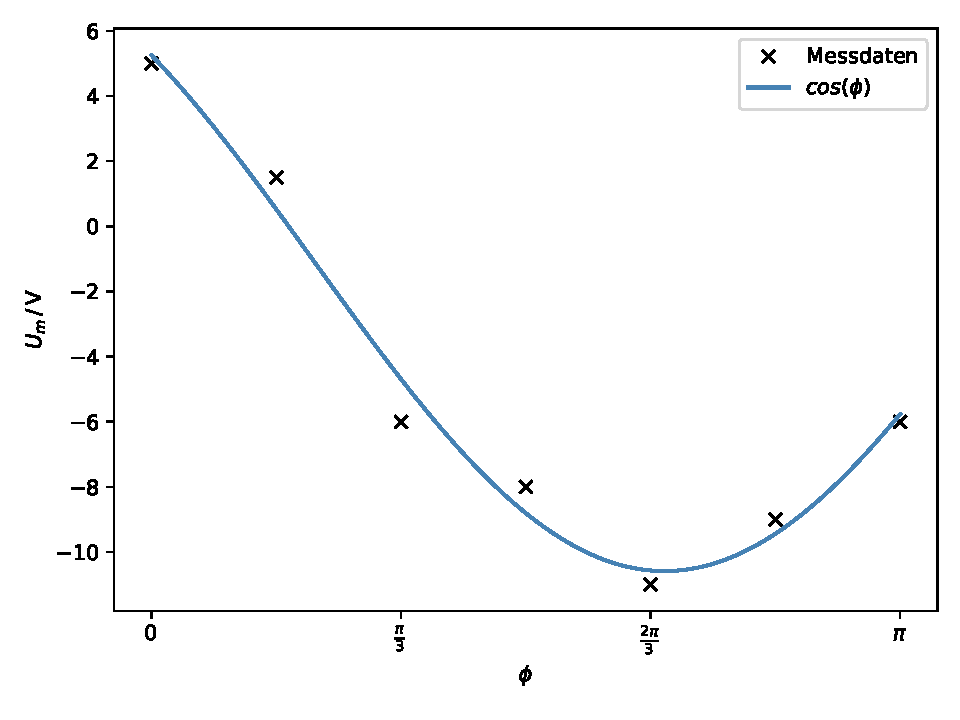
\includegraphics[height=6.9cm]{Daten/phasenoise.pdf}
  \caption{Spannungsamplituden in Abhängigkeit von $\phi$ mit Rauschen.}
  \label{fig:phasenoise}
\end{figure}

\newpage
\noindent
Um die cosinus-Abhängigkeit aus Formel (\ref{eqn:uout2}) zu untersuchen, wird mittels Python ein fit der Funktion 

\begin{equation*}
f(\phi) = a \cdot cos(b \cdot \phi + c) + d
\label{eqn:cos}
\end{equation*}

\noindent
durchgeführt.
Dabei ergeben sich folgende Parameter für den fit ohne Rauschen (\ref{fig:phase}) und mit Rauschen (\ref{fig:phasenoise}):

\begin{align*}
\text{ohne}&\text{ Rauschen} & \text{mit}& \text{ Rauschen} \\
a &= 61.86 & a &= 9.51\\
b &= 1.05  & b &= 1.07\\
c &= 1.05  & c &= 0.84\\
d &= 0.64  & d &= -1.07\\
\end{align*}

\noindent


\subsection{Untersuchung der Photodiode}
Aus der Messung ergeben sich folgende Werte:

\begin{table}
  \centering
  \begin{tabular}{c c}
  \toprule
  {$d \mathbin{/} \si{\centi\meter} $} & {$U \mathbin{/} \si{\volt} $}\\
  \midrule
  4.55 &   25\\
  5    &  23\\
  6    &  19\\
  7    &  16\\
  8    &  14\\
  9    &  12\\
  10   &   10\\
  11   &   9\\
  12   &   7.8\\
  13   &   6.8\\
  14   &   6\\
  15   &   5.5\\
  16   &   5\\
  17   &   4.5\\
  22   &   2.9\\
  27   &   2\\
  32   &   1.8\\
  37   &   1.6\\
  \bottomrule
  \end{tabular}
  \caption{Spannung in Abhängigkeit des Abstands zum Detektor.}
  \label{tab:led}
  \end{table}

\noindent
Die Messwerte werden aufgetragen und mit verschiedenen Funktionen gefittet.
So ergegen sich folgende Parameter der Fitfunktionen:

\begin{align*}
  f(d) &= \frac{a}{r} + b & f(d)&= \frac{a}{r^2} + b \\
  a &= 1.28   & a &= 0.05\\
  b &= -2.67  & b &= 3.39\\
  \end{align*}

  \begin{figure}
    \centering
    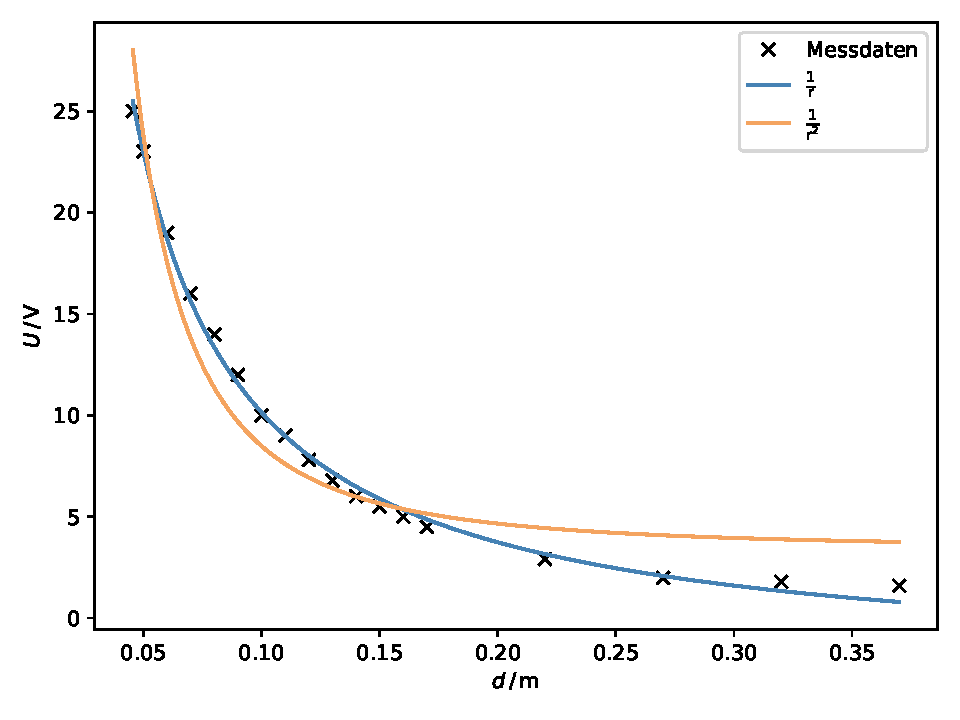
\includegraphics[height=9cm]{Daten/led.pdf}
    \caption{Spannung in Abhängigkeit des Abstands zum Detektor.}
    \label{fig:led}
  \end{figure}